\documentclass{article}
%\documentclass[conference]{IEEEtran}
\usepackage[utf8]{inputenc}
\usepackage[english]{babel}
\usepackage{ragged2e}
\usepackage{blindtext}
\usepackage{geometry}
\usepackage{authblk}
\usepackage{comment}
\usepackage{rotating}
\usepackage{float}
\usepackage{amsmath}
\usepackage{amsfonts}
\usepackage{booktabs}
\usepackage{pifont}
 \usepackage{graphicx,caption,subcaption}
    \captionsetup[subfigure]{labelformat=simple}
\usepackage{amssymb}
\usepackage{algpseudocode}
\usepackage{scrextend}
\usepackage{caption}
\usepackage{subcaption}
\usepackage{threeparttable}
\usepackage{multicol}
\usepackage{lipsum}
\usepackage{booktabs, caption, makecell}
\usepackage{multirow}
\usepackage{tabularx}
\usepackage{graphicx}
\usepackage{subfigure}
\usepackage{caption}
\usepackage{biblatex}
\usepackage{authblk}
\usepackage{algorithm}
\usepackage{algpseudocode}
\usepackage[pdfborder={0 0 0}]{hyperref}% For email addresses
\setlength{\columnsep}{1cm}


 \geometry{
 a4paper,
 total={170mm,257mm},
 left=20mm,
 top=20mm,
 }

\title{\Large\textbf{SimAN: Exploring Self-Supervised Representation Learning of Scene Text
via Similarity-Aware Normalization}\\

}
% Authors
\author[1]{\textbf{ Canjie Luo}}
\author[1,2,*]{\textbf{ Lianwen Jin} }
\author[3]{\textbf{Jingdong Chen}}


% Author Affiliations
% \affil[1]{South China University of Technology \\
% \url{jingdongchen.cjd@antgroup.com}}
% \affil[2]{Google Research, Brain Team}
{
\makeatletter
    \renewcommand\AB@affilsepx{\protect\Affilfont}
    \makeatother

    \makeatletter
    \renewcommand\AB@affilsepx{, \protect\Affilfont}
    \makeatother

    \affil[1]{South China University of Technology}
    \affil[2]{Peng Cheng Laboratory}
    \affil[3]{Ant Group}
}
\date{\vspace{-8ex}}

\addbibresource{bib.bib} 
\begin{document}
\maketitle

\begin{center}
    \textmd{\texttt{\{canjie.luo, lianwen.jin\}@gmail.com,jingdongchen.cjd@antgroup.com}}
\end{center}


\begin{multicols}{2}

\begin{abstract}
\textit{Recently self-supervised representation learning has
drawn considerable attention from the scene text recognition community. Different from previous studies using contrastive learning, we tackle the issue from an alternative
perspective, i.e., by formulating the representation learning
scheme in a generative manner. Typically, the neighboring image patches among one text line tend to have similar styles, including the strokes, textures, colors, etc. Motivated by this common sense, we augment one image patch
and use its neighboring patch as guidance to recover itself.
Specifically, we propose a \underline{Sim}ilarity-\underline{A}ware \underline{N}ormalization
(SimAN) module to identify the different patterns and align
the corresponding styles from the guiding patch. In this
way, the network gains representation capability for distinguishing complex patterns such as messy strokes and cluttered backgrounds. Experiments show that the proposed
SimAN significantly improves the representation quality and
achieves promising performance. Moreover, we surprisingly find that our self-supervised generative network has
impressive potential for data synthesis, text image editing,
and font interpolation, which suggests that the proposed
SimAN has a wide range of practical applications.}
\end{abstract}

\section{Introduction}

The computer vision community has witnessed the great
success of supervised learning over the last decade. However, the supervised learning methods heavily rely on
labor-intensive and expensive annotations. Otherwise, they
might suffer from generalization problems. Recently selfsupervised representation learning has become a promising
alternative and is thus attracting growing interest [24,34]. It
has been shown that the self-supervised representations can
benefit subsequent supervised tasks [6–10, 18].
Despite the fast-paced improvements of representation
learning on single object recognition/classification tasks

\begin{figure}[H]
     \centering
     \begin{subfigure}[t]{0.5\textwidth}
         \centering
         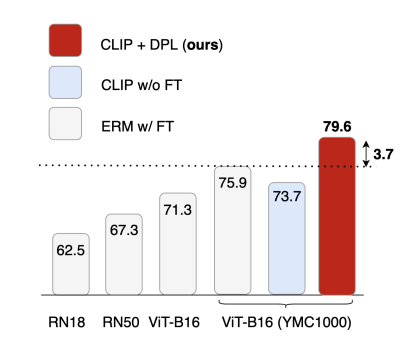
\includegraphics[width= \textwidth]{1.png}
         \caption{Contrastive representation learning}
         \label{fig:Figure_1}
     \end{subfigure}
     \begin{subfigure}[t]{0.5\textwidth}
         \centering
         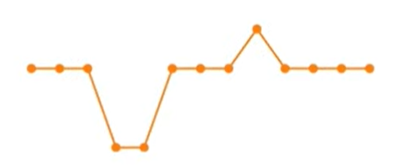
\includegraphics[width=\textwidth]{2.png}
         \caption{Generative representation learning (ours) }
         \label{fig:Figure_2}
     \end{subfigure}
    

        \caption{Scene text representation learning in (a) the contrastive
and (b) the generative manner (ours). We estimate the similarity
of the content representations between the augmented patch and
its neighboring patch, and align the corresponding styles to reconstruct the augmented patch. Only high-quality representations are
distinguishable so that a precise reconstruction can be achieved}
        \label{fig:whole_1}

\end{figure}
 The learning scheme is shown in Figure \ref{fig:Figure_1}.

To summarize, our contributions are as follows:

\begin{itemize}
    \item We propose a generative (opposite of contrastive [34])
representation learning scheme by utilizing the unique
properties of scene text, which might inspire rethinking the learning of better representations for sequential
data like text images. To the best of our knowledge,
this is the first attempt for scene text recognition.

   \item  We propose a SimAN module, which estimates the
similarity of the representations between the augmented image patch and its neighboring patch to align
corresponding styles. Only if the representations are
sufficiently distinguishable, different patterns can be
identified and be aligned with correct styles. Otherwise, the network might result in a wrong recovered
image, e.g., in different colors.

\item  The proposed SimAN achieves promising representation performance. Moreover, the self-supervised network shows impressive capabilities to synthesize data,
edit text images and interpolate fonts, suggesting the
broad practical applications of the proposed approach.

\end{itemize}

\begin{comment}
    \begin{center}
\captionof{table}{Arbitrary-length Text editing evaluation. We report FID
score and word-level recognition accuracy (\%). Although the supervised EditText can imitate more font category and background
texture, our self-supervised approach achieves better readability}
\begin{tabular}{ c c c c } 

 \hline
 Method & Supervision & FID & Acc. \\
 \hline
 EditText & \checkmark & \textbf{40.5} & 14.9 \\ 
 Ours & $\times$ & 67.9 & \textbf{57.6}  \\ 
 \hline
\end{tabular}
\end{center}
\end{comment}

\section{Related Work}
\subsection{ Data Hunger of Scene Text Recognition}
Scene text recognition is a crucial research topic in the
computer vision community, because the text in images provides considerable semantic information for us. One important open issue in this field is data hunger. Typically,
mainstream scene text recognizers [14, 45, 54] require a
large number of annotated data. However, data collection
and annotation cost a lot of resources. For instance, annotating a text string is tougher than selecting one option
as the ground truth for single object classification datasets,
whereas tens of millions of training data are required to gain
robustness. Although synthetic data are available, previous
studies [26,33,37,61] suggested that there is a gap between
real and synthetic data. To mitigate this problem, Zhang et
al. [61] and Kang et al. [26] proposed domain adaptation
models to utilize unlabeled real data. Our study explores
representation learning in a generative way, which is an alternative solution to make use of unlabeled real da
\subsection{Visual Representation Learning}
In the big data era, tremendous amounts of unlabeled
data are available. Making the best use of unlabeled data becomes a crucial topic. Self-supervised representation learning has drawn massive attention owing to its excellent capability of pre-trained feature extraction [24, 34]. For instance, an encoder trained after a pretext task can extract
transferrable features to benefit downstream tasks. We summarize popular methods into two main categories according
to their objectives as follows.
The contrastive learning scheme defines the pretext
task as a classification task or a distance measuring task. For
instance, the pretext task is to predict relative rotation [31]
and position [56]. Recently the similarity measuring pretext task has become dominant, which aims to minimize
the distance between the positive pairs while maximizing
their distance to the negative ones using a discriminative
head [5, 7, 8, 10, 18]. It is closely related to metric learning.
Furthermore, the similarity measuring task using only positive pairs and discarding negative samples [9, 16] is also emerging topic.
For the field of scene text, Baek et al. [3] introduced existing self-supervised techniques [18, 31] to use unlabeled
data but resulted in approximately the same performance.
Aberdam et al. [1] proposed a contrastive representation
learning scheme, termed SeqCLR, to satisfy the sequenceto-sequence structure of scene text recognition. This is the
first step towards scene text representation.
The generative learning scheme has not been intensively studied in computer vision. One reason for this may
be that the raw image signal is in a continuous and highdimensional space, unlike the natural language sentences in
a discrete space (e.g., words or phrases) [18]. Therefore, it
is difficult to define an instance. Although it is possible to
model the image pixel by pixel [50], this theoretically requires much more high-performance clusters [6]. Another
solution is the denoising auto-encoder [49,52], which learns
features by reconstructing the (corrupted) input image.
Our approach falls into the second category of visual representation learning, i.e., the generative learning scheme.
We propose a novel representation learning scheme by
studying the unique properties of scene text and using an
image reconstruction pretext task
\pagebreak
\end{multicols}
\begin{figure}[H]
         \centering
         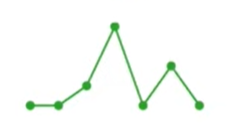
\includegraphics[width=\textwidth]{3.png}
         \label{fig:three}
         \caption{Overview of the proposed generative representation learning scheme. We decouple content and style as two different inputs and
guide the network to recover the augmented image. The proposed SimAN module learns to align corresponding styles for different patterns
according to the distinguishable representations.}
\end{figure}
\begin{multicols}{2}

\section{Methodology}
In this section, we first introduce the design of the pretext
task and the construction of the training samples. Then, we
detail the proposed SimAN module. Finally, we present the
objectives of the task and the complete learning scheme.
The overall framework is shown in Figure 2  

\subsection{Training Sample Construction}
Constructing appropriate training samples is critical to
the success of the pretext task. We enable the scene text
representation learning by recovering an augmented image
patch using its neighboring patch as guidance. This design
considers the unique properties of scene text, i.e., the styles
(e.g., stroke width, textures, and colors) within one text line
tend to be consistent.\\
The pretext task requires decoupled style and content inputs. As shown in Figure 2, given an unlabeled text image
I ∈ R
3×H×W (the width W is required to be larger than
two times of height H), we randomly crop two neighboring image patches Is, Ic ∈ R
3×H×H as style and content
input, respectively. This ensures sufficient differences in
content between the two patches. Even if the neighboring
patches might contain a same characters, their positions are
different. Then, we augment (blurring, random noise, color
changes, etc.) the content patch Ic as Iaug to make its style
different from the style patch Is. Finally, the pretext task
takes Iaug as content input and Is as the style guidance to
recover an image Irec. The source content patch Ic serves
as supervision.\\
\textbf{Discussion} As our pretext task is recovering an augmented patch under the guidance of its neighboring patch,
the visual cues should be consistent in both patches. Some
spatial augmentation strategies, such as elastic transformation, might break the consistency and lead to failed training.
For instance, it might bring changes to the stroke width.
The excessively distorted strokes are also diverse from the
source font style. Therefore, we avoid all of the spatial
transformation augmentation methods that are widely used
for self-supervised representation learning. This is also a
significant difference with previous study SeqCLR \cite{aberdam2021sequence}



\subsection{Similarity-Aware Normalization}
Previous studies [\cite{huang2017arbitrary}, \cite{karras2019style}] revealed that the statistics of
feature maps, including mean and variance, can represent
styles. Based on this finding, we perform instance normalization (IN) [\cite{huang2017arbitrary},\cite{ulyanov2016instance}] on the feature maps to remove the style

\begin{equation}
    \sigma_{\textit{c,i,j}} = 
    \frac{1}{3}\sqrt{\sum\nolimits_{p,q \in \mathcal{N}_{i,j}} (x_{c,p,q}-\mu_{c,i,j})^2}
\end{equation}

\subsection{Learning Scheme}
As we formulate the pretext task as image reconstruction, the source patch $I_c$ can serves as supervision. We minimize the distance between the recovered image $I_rec$ and
target image $I_c$ as
\begin{equation}
    \small \mathcal {L}_2 = \| I_{rec} - I_c \|_{2}^{2}
\end{equation}
 
Simultaneously, we adopt a widely used adversarial objective to minimize the distribution shift between the generated and real data:
\begin{equation}
     \small \min _{D} \mathcal {L}_{adv}=\mathbb {E} \big [ \big (D (I_s)-1 \big )^{2} ]+\mathbb {E} [ \big (D (I_{rec} ) \big )^{2} \big ], 

\end{equation}
\begin{equation}
     \small \min _{\text {Encoder, Decoder }} \mathcal {L}_{adv}=\mathbb {E}\big [ (D (I_{rec})-1\big )^{2}\big ], 
\end{equation}

where D denotes a discriminator.\\
The complete learning scheme is shown in Algorithm 1.
The encoder/decoder and discriminator are alternately optimized to achieve adversarial training.


\begin{algorithm}[H]
    \caption{Representation Learning Scheme}
    \label{algo_2}
    \begin{algorithmic}[1]
    \Require  Encoder, Decoder, Discriminator D
    \Ensure  Encoder, Decoder
    \For {iteration t = 0,1,2,\dots,T}
    \State Sample a mini-batch ${{\{I_i\}}^B}_{i=1}$ from unlabeled data
    \For {each $ I_i $}
    \State Randomly crop Is and Ic, augment Ic as Iaug 
    \EndFor
    \State Forward Encoder, SimAN and Decoder
    \State Compute loss for  ${{\{I_{rec,i}\}}^B}_{i=1}$
    \State Update D using $\underset{D}{min }  \mathcal {L}_{adv}$
    \State : Update Encoder and Decoder using \\
              $\small \underset{\text {Encoder, Decoder }}{min} \mathcal {L}_{adv} + \lambda\mathcal{L}_2 $
    \end{algorithmic}
\end{algorithm}

\section{Experiments}
\subsection{ Dataset}
\subsection{Implementation Details}
\hspace{5pt} We provide more details, such as augmentations, architectures, probe objectives, and training settings, in the \textit{Supplementary Material}.\\
 \hspace{5pt} \textbf{Encoder/Decoder} We adopt a popular recognizer backbone ResNet-29 [2] as our encoder. We symmetrically design a lightweight decoder.\\
\hspace{5pt} \textbf{Recognizer} The complete architecture of the recognizer
follows [1,2], including a rectification module, a ResNet-29
backbone, two stacked BiLSTMs and a CTC [15] /Attention [4] decoder, as shown in Figure 3.\\
\hspace{5pt} \textbf{Optimization} In the self-supervised representation
learning stage, we set the batch size to 256 and train the
network for 400K iterations. It takes less than 3 days for
convergence on two NVIDIA P100 GPUs (16GB memory
per GPU). The optimizer is Adam [30] with the settings
of $\beta1 = 0.5$ and $\beta2 = 0.999$. The learning rate is set to
10−4
and linearly decreased to 10−5
. The images are resized to a height of 32 pixels, maintaining the aspect ratio.
The training setting of recognizers follows previous study
SeqCLR [1].

\subsection{ Probe Evaluation}
Moreover, we find that this experimental setting (pretraining the backbone and fine-tuning the probe using the
very same synthetic dataset) might not meet the actual practice. In fact, we usually encounter one situation that we
have vast amounts of unlabeled real-world data. It is worth
making the best use of the real-world data. Therefore, we
conduct an experiment under this new setting to further verify the effectiveness of our approach. We perform selfsupervised learning of the backbone using the Real-300K
dataset. As shown in Table \ref{tab:example}, the recognition performance
is significantly boosted. As the real-world dataset provides
more realistic and diverse images, it benefits the robustness
of the backbone.
% @{}lllccccc@{}
\begin{table}[H]
  \centering
  \caption{Probe evaluation. We report the word accuracy (Acc., %)
and word-level accuracy up to one edit distance (E.D. 1, %). The
real training data provides more robust representations.}
  \label{tab:example} 
  \scalebox{0.8}{
  \begin{tabular}{ccccccccc}
    \toprule
   \small Probe & \multicolumn{2}{c}{\small Training Data} & \multicolumn{2}{c}{\small IIIT5K} & \multicolumn{2}{c}{\small IC03} & \multicolumn{2}{c}{\small IC13} \\
    \cmidrule(lr){2-3}
    \cmidrule(lr){4-5}
    \cmidrule(lr){6-7}
    \cmidrule(lr){8-9}
    \small Type & \small Encoder & \small Probe & \small Acc. & \small E.D.1 & \small Acc. & \small E.D.1 & \small Acc. & \small E.D.1  \\
    \midrule
    \multirow{2}{*}{CTC} & \small Synth. & \small Synth. & 60.8 & 75.6 & 64.9 & 78.9 & 64.0 & 81.0 \\
     & \small Real & \small Synth. & \textbf{68.8} & \textbf{82.6} & \textbf{75.9} & \textbf{87.9} & \textbf{74.0} & \textbf{86.0} \\
     \hline
    \multirow{2}{*}{Att.} & \small Synth. & \small Synth. & 66.8 & 78.6 & 71.9 & 83.9 & 68.6 & 81.7 \\
     & \small Real & \small Synth. & \textbf{73.8} & \textbf{85.6} & \textbf{81.9} & \textbf{90.9} & \textbf{77.0} & \textbf{87.8} \\
    \bottomrule
  \end{tabular}}
\end{table}
\subsection{ Semi-Supervision Evaluation}
\subsection{ Generative Visual Tasks}
\subsubsection{ Data Synthesis}


% \begin{figure}[H]
%          \centering
%          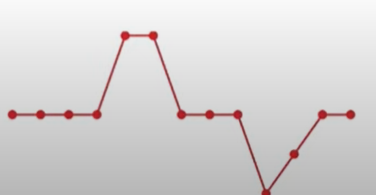
\includegraphics[width=0.5\textwidth]{4.png}
%          \label{fig:4}
%          \caption{Distribution of scene text images containing the word
% “the” via t-SNE. We show two distributions of (a) 200 real labeled
% samples and (b) 200 real samples and our 2000 synthetic samples.
% The large empty space of original distribution might suggest the
% lack of diversity of labeled data. After adding our synthetic samples, the distribution is more even and dense. Best viewed in color}
% \end{figure}

\begin{figure}[H]
     \centering
     \begin{minipage}[b]{0.23\textwidth}
         \centering
         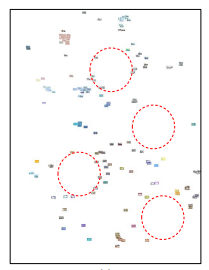
\includegraphics[width=\textwidth]{5.png}
         \caption*{(a)}
         \label{fig:Figure_5}
     \end{minipage}
     \hfill
     \begin{minipage}[b]{0.23\textwidth}
         \centering
         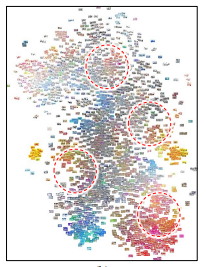
\includegraphics[width=\textwidth]{6.png}
         \caption*{(b)}
         \label{fig:Figure_6}
     \end{minipage}
    

        \caption{Distribution of scene text images containing the word
“the” via t-SNE. We show two distributions of (a) 200 real labeled
samples and (b) 200 real samples and our 2000 synthetic samples.
The large empty space of original distribution might suggest the
lack of diversity of labeled data. After adding our synthetic samples, the distribution is more even and dense. Best viewed in color}
         \label{fig:whole_5}

 \end{figure}

 First, we visualize the distributions of the limited real
labeled samples and our plentiful synthetic samples. As
shown in Figure \ref{fig:whole_5}, the limited labeled real-world data cannot cover diverse styles. However, our synthetic data fills
the empty style space, indicating the significantly enriched
styles. Then, we conduct recognition experiments to show
the quantitative results

\subsubsection{Arbitrary-Length Text Editing}

The goal of editing text in the wild is to change the word on
the source image while retaining the realistic source look.
As our approach can synthesize new words within source
styles, we study the performance of our self-supervised approach and a popular supervised method EditText
[57]. We
generate 10K images using the corpus of SynthText [17]
and the style of IC13 [28]. Then we evaluate the style distribution similarity using the FID score [20] and the readability using a mainstream recognizer3
[44]. As shown in Table \ref{tab:tab_6}, the EditText cannot handle target text
of various lengths.

    \begin{center}
\captionof{table}{Arbitrary-length Text editing evaluation. We report FID
score and word-level recognition accuracy (\%). Although the supervised EditText can imitate more font category and background
texture, our self-supervised approach achieves better readability}
\label{tab:tab_6}
\begin{tabular}{ c c c c } 

 \hline
 Method & Supervision & FID\downarrow & Acc.\uparrow \\
 \hline
 EditText & \checkmark & \textbf{40.5} & 14.9 \\ 
 Ours & $\times$ & 67.9 & \textbf{57.6}  \\ 
 \hline
\end{tabular}
\end{center}

\section*{Acknowledgement}

\hspace{5pt} This research was supported in part by NSFC (Grant No.
61936003) and GD-NSF (No. 2017A030312006).

% \end{multicols}

% \begin{table}[h!]
% %\begin{threeparttable}
%     \centering
%     \caption{Multi col table}
    
%     \begin{tabularx}{0.8\textwidth}{|c|c|c|c|}
%         \hline
%         \multirow{10}{*}{numeric literals} & \multirow{5}{*}{integers} & in decimal & 8743\\
%         \hline
%         & &  \multirow{2}{*}{in octal} & 7464\\
%         \hline
%         & & & 103\\
%         \multirow{2}{*}{4}  & 5 & 6\\
%         \cline{3-4}
        
%         \hline
%         \multicolumn{2}{|c|}{\multirow{2}{*}{10}} & 12\\
%         \cline{3-3}
%         \multicolumn{2}{|c|}{} & 17 \\
%         \hline
        
%     \end{tabularx}
%     \begin{tablenotes}
%       \item[1] Note that \textit{Getting On Sequence} will start from steady standing in the station.
%       \item[2] Note that \textit{Getting Off Sequence} will start from steady sitting state in the Tram.
%    \end{tablenotes}
%     \label{tab:Multi col table}
%     %\end{threeparttable}
% \end{table}


% \begin{equation}
%     x = \frac{\sqrt{\sin{\theta}}+{\cos{\theta}}+T_i}{e^{-20}}
% \end{equation}


% \begin{equation}
%     p_{ap}^{i} = 
%     \frac{1}{N} = \sum_{j=1}^{N}F(f(x_{j}^{i}))
% \end{equation}



% \begin{comment}
% \begin{center}
%     \Large
%     \textbf{Thesis Title}
        
%     \vspace{0.4cm}
%     \large
%     Thesis Subtitle
        
%     \vspace{0.4cm}
%     \textbf{Author Name}
 
%     \vspace{0.9cm}
%     \begin{flushleft}
%     \textbf{Abstract}
%     \item[\textbf{Motivation :}]
%     \item[\textbf{Results :}]
%     \end{flushleft}
% \end{center}
% \end{comment}
% \begin{multicols}{2}

% \pagebreak
% \begin{figure}[H]
%          \centering
%          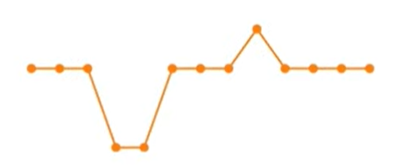
\includegraphics[width=0.5\textwidth]{2.png}
%          \label{fig:three sin x}
%          \caption{Accuracy of SAINT-base and MUFOLD-SS under various levels of non-local interactions. We show the results on the TEST2016 test set using six bins of proteins}
% \end{figure}
% \begin{figure}[H]
%          \centering
%          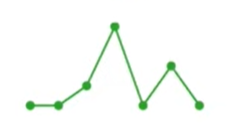
\includegraphics[width=0.5\textwidth]{3.png}
%          \label{fig:three sin x}
%          \caption{. Accuracy of SAINT, SPOT-1D, NetSurfP-2.0 and MUFOLD-SS as a function of the average number of non-local interactions per residue. We show the results on the six bins as shown in Table 6}
% \end{figure}

\begin{comment}
    \begin{wrapfigure}{l}{0.25\textwidth}
\includegraphics[width=0.9\linewidth]{overleaf-logo} 
\caption{Caption1}
\label{fig:wrapfig}
\end{wrapfigure}
\end{comment}


\end{multicols}

% \begin{table}[H]
%     \centering %table will be in the middle
%     \begin{tabular}{|c |c| c| c| } %c means cell content will be center aligned, l means left aligned, r means right aligned | means divider between columns
%          \hline
%          \multirow{10}{*}{numeric literals} & \multirow{5}{*}{integers} & in decimal & 8743 \\
%          %\hline %horizontal line
%          \cline{3-4}
%          % \cline{4-5}
%          %\cmidrule(lr){2-3} \cmidrule(lr){4-5}
%          %\hline{4-5}
%          & & \multirow{2}{*}{in octal} & 7464\\
%          \cline{4-4}
%          & &  & 103\\
%          \cline{3-4}
%          & & \multirow{2}{*}{in hexadecimal} & 5A0FF\\
%          \cline{4-4}
%          & &  & E0F2\\
%          \cline{2-4}
%          & \multirow{5}{*}{fractions} & \multirow{5}{*}{in decimals}  & 140.58\\
%          \cline{4-4}
          
%          & & & 8.04\\
%          \cline{4-4}
%          & & & 0.34\\
%          \cline{4-4}
%          & & & 5.47\\
%          \cline{4-4}
%          & & & 47e22\\
%          \hline
%          \multirow{3}{*}{char literals} & \multirow{3}{*}{} & \multirow{3}{*}{} & 'H' \\
%          \cline{4-4}
%          & & & '\backslash n'\\
%          \cline{4-4}
%          & & & '\backslash x64'\\
%          \hline
          

%     \end{tabular}
%     \caption{Multi column table}
%     \label{tab:multicol} %to refer this table
% \end{table}


\printbibliography
\end{document}
